\documentclass[a4paper,11pt,singlespacing]{article}

\usepackage{setspace}
\usepackage[utf8]{inputenc}
\usepackage[T1]{fontenc}
\usepackage{graphicx}
\usepackage{color}
\usepackage{hyperref}
\usepackage{listings,xcolor}

\graphicspath{ {./images/} }

\title{Projektskizze: WLAN-AP mit regelmäßigem PSK-Tausch und RFID-Anmeldung}
\date{\today}

\begin{document}
	\setlength{\parindent}{0ex}
	
	\maketitle
	
	\section{Motivation}
	Der Hauptgrund für dieses Projekt war der umständliche Prozess der Anmeldung von Gästen im Wlan mit einem sicheren pre-shared Key. Dieser Key sollte aufgrund der Sicherheit lang und kryptisch gewählt sein, somit muss man ihn bei jeder Anmeldung neu heraussuchen und eintippen. Zudem behalten die Gäste den Zugang zum Netzwerk, obwohl man das nicht möchte. Der Vorgang den Schlüssel manuell zu ändern ist zeitaufwendig und unnötig. Deshalb soll mit diesem Projekt dieser Vorgang vereinfacht und komfortabler gemacht werden. 
	
	\section{Problem}
	Der pre-shared Key eines WLAN-Netzwerkes wird in den meisten Heimnetzwerken einmal oder gar nicht geändert. Dies hat zur Folge, dass sobald einmal das Passwort geknackt oder bewusst/unbewusst weitergegeben wurde, sich jeder mit dem Access-Point verbinden kann. Regelmäßiges Wechseln des Keys führt jedoch zu unangenehmen Mehraufwand, den sehr viele Nutzer nicht eingehen wollen. Die Folge sind ungewollte Endgeräte im eigenen Heimnetz.

	\section{Lösungsansätze}
	Ein Lösungsansatz stellt ein sich automatisch oder auf Tastendruck ändernder pre-shared Key dar. Mit diesem können sich Endgeräte anmelden und kommunizieren. Hiermit wird das Problem der ungewollten Nutzern gelöst, denn diese können sich sobald der Key gewechselt hat, nicht mehr im Netz anmelden. Der Key wird an einem Display in zwei verschiedenen Varianten angezeigt:
	\begin{itemize}
		\item Klartext für Endgeräte ohne Kamera z.B. Laptops oder Drucker
		\item QR-Code zum Scannen für z.B Smartphones
	\end{itemize}
	Es wurde sich für einen QR-Code anstatt eines RFID/NFC Transponder entschieden, da hier die Möglichkeit des Abgreifens des Schlüssel nicht besteht. 

	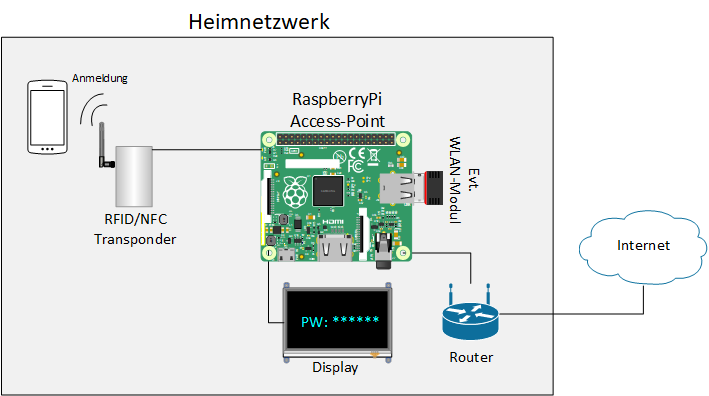
\includegraphics[scale=0.6]{skizze}
	
	\section{Anforderungsanalyse}

	Für dieses Projekt wird ein Raspberry Pi 3 B oder 3 B+ benötigt. Grund hierfür ist der HDMI Anschlusses, der aus komfort Gründen für den Display benutzt werden soll. Zudem hat dieses Modell ausreichend Leistung, ein integriertes WLAN-Modul und alle nötigen Anschlüsse(z.B. Pins für Taster/Umschalter, LAN-Anschluss). \\
	Das Display, das verwendet wird, muss eine ausreichende Auflösung für die Darstellung des QR - Codes besitzen. Deshalb können keine der kleineren und billigeren LCD Anzeigen verwendet werden. Außerdem muss diese noch an den Raspberry Pi in Form von HDMI angeschlossen werden, da die Pins für mögliche Schalter/Umschalter verwendet werden. \\
	Zu Testzwecken werden unterschiedliche Smartphones (Android/iOS) und Notebooks benutzt. So soll Sichergestellt werden, dass mögliche Probleme aufgrund von Diskrepanzen zwischen den Betriebssystemen bzw. Hardware erkannt werden.\\
	Um den Raspberry als Access Point verwenden zu können, müssen zusätzliche Pakete installiert und eine Netzwerkkonfiguration vorgenommen werden. Darunter fällt das Einstellen von DHCP und DNS für die Clients, sowie das erzeugen des pre-shared Key. Weiterhin muss eine eine Passwortrichtlinie festgelegt werden. In dieser wird vor allem die Länge und die Art der Verschlüsselung definiert.\\
	Als Skriptsprache empfiehlt sich Python, da es sehr viele Libraries gibt, die einiges an Arbeit abnehmen. Für die QR-Code Generierung eignen sich die Libraries qrcode und PyQRCode. Für die Generierung eines Schlüssels sollte nach einer passenden Library gesucht werden.\\
	Zum Schluss muss geschaut werden, wie der neu generierte pre-shared Key ausgetauscht werden kann.\\
	
	\section{Priorisierung}
	
	Das wichtigste zu Beginn ist, dass die Hardware aufeinander abgestimmt wird. Bedeutet, alle Teile passen zusammen und können angeschlossen werden.\\
	Danach muss die Konfiguration des Raspberry Pi zum Access Point erfolgen. Sobald dies funktioniert kann das Generieren des pre-shared Keys und dessen Austausch stattfinden. Folglich wird die Ausgabe des Keys am Bildschirm realisiert. Danach kann dies, um das Generieren des QR-Codes und dessen Ausgabe erweitert werden.\\
	Wenn diese Punkte voll funktional umgesetzt werden konnten, kann sich um einen automatischen oder manuellen Job (bei Tastendruck) zum Generieren und Austauschen des Keys gekümmert werden.
	
\end{document}
